\documentclass[11pt]{report}
\usepackage{amsmath}
\usepackage[margin=1in, paperwidth=8.5in, paperheight=11in]{geometry}
\usepackage{graphicx}
\usepackage{listings}
\usepackage{minted}
\usepackage[usenames, dvipsnames]{xcolor}
\definecolor{mygray}{gray}{0.9}
\date{} 

\begin{document}

\font\myfont=cmr12 at 45pt

\title{{\textbf{\myfont Channel Coding}}}
\maketitle

\chapter{BER for BPSK in AWGN with Hamming (7,4) code}

\section{Overview}

\Large{
We'll be discussing sections of a code that encodes the input data using Hamming (7,4) code, and then decodes it after the data is simulated to be transmitted through a AWGN channel using BPSK modulation.}

\section{Encoder}
\Large{
The first part of the code is the encoder. Firstly, we define the hamming code parity check matrix and the generator matrix, and subsequently generate a codebook by coding all 16 possible combinations of the 4 data bits using the generator matrix. }\\

\begin{minted}
[frame=lines,
bgcolor=mygray,
]
{python}
import numpy as np
ht=np.matrix([[1,1,1],[1,0,1],[1,1,0],[0,1,1],
             [1,0,0],[0,1,0],[0,0,1]])
g=np.matrix([[1,0,0,0,1,1,1],[0,1,0,0,1,0,1],
             [0,0,1,0,1,1,0],[0,0,0,1,0,1,1]])

for kk in range(2**4):
    m_vec=np.matrix(map(int,np.binary_repr(kk,width=4)))
    c_vec[kk,:]=(m_vec*g)%2
\end{minted}
\\

\Large{
Subsequently, random bits of data are encoded using the generator matrix, and BPSK modulation is used. N = $\mathrm{2}*10^6$ bits are used and an array \textit{ip} is used to store the random bits. The function \textit{randint} of the numpy package is used to generate the data. The array is rearranged into a matrix and encoded using the generator matrix. The encoded data is reshaped again before BPSK modulation is used for sending the data. \textit{Eb\_N0\_db} is the SNR range from 1 to 11 dB.}
\\

\begin{minted}
[frame=lines,
bgcolor=mygray,
]
{python}
N=2*(10**6)  #number of bits
Eb_N0_dB=np.arange(0,11,1)
Ec_N0_dB=Eb_N0_dB - 10*np.log10(7.0/4)
for yy in range(len(Eb_N0_dB)): 
    
    #transmitter
    ip = np.random.randint(2,size=N)
    ip=np.array(ip)
       
        #hamming coding (7,4)
    ipM=np.matrix(np.reshape(ip,(-1,4)))
    ipC=(ipM*g)%2
    cip=np.reshape(ipC,(1,(N/4)*7))
        
        #BPSK modulation
    s=2*cip-1    
\end{minted}
\\

\Large{
The above \textit{for} loop is continued, and White Gaussian Noise is generated and added to the Modulated signal. }\\

\begin{minted}
[frame=lines,
bgcolor=mygray,
]
{python}
    sigma = np.sqrt((1/2.0)*(10**(-Ec_N0_dB[yy]/10)))
    n=np.random.normal(0,sigma,(np.shape(cip)))
    #noise addition to the modulated signal
    y=s+n   
    y=np.array(y)    
\end{minted}
\\

\section{Decoder}
\Large{The received bits can be decoded using the hard hamming decoder, or the soft Hamming decoder.}


\subsection{Hard Decoder}
\Large{
First, the positive values of the received data are identified, and the syndrome of the received data is calculated using the Parity Check matrix after the data is rearranged.
}

\begin{minted}
[frame=lines,
bgcolor=mygray,
]
{python}
    cipHard=(y>0)*1
    cipHardM = np.matrix(np.reshape(cipHard,(-1,7)))
    syndrome = (cipHardM*ht)%2
    syndrome = np.array(syndrome).astype(int)
    a=np.array([[4,2,1]])
    a=np.reshape(np.tile(a,N/4),(N/4,3))
    syndromeDec =np.sum(syndrome*a,axis=1) 
\end{minted}
\\

\Large{For proceeding further, a bit index matrix \textit{bitIdx} = [7,7,4,7,1,3,2] is defined outside the \textit{for} loop. The index of the error bits is found using the syndrome matrix and the bits are corrected.}\\


\begin{minted}
[frame=lines,
bgcolor=mygray,
]
{python}
    bitIdx=np.array(bitIdx)
    bitCorrIdx = bitIdx[syndromeDec-1] 
    bitCorrIdx = bitCorrIdx + np.arange(0,N/4,1)*7  
    cipHard[0,bitCorrIdx-1] = 1-cipHard[0,bitCorrIdx-1] 
\end{minted}
\\

\Large{An index for the overall data bits is defined using two matrices, a1 and b1 and the corresponding data bits are identified, which is shown as the 'sent data' by the decoder.}


\begin{minted}
[frame=lines,
bgcolor=mygray,
]
{python}
    a1 = np.arange(1,5,1)
    a1 = np.tile(a1,N/4)
    b1 = np.repeat(np.arange(0,N/4)*7,4)
    idx = a1+b1   # index of data bits
    ipHat_hard = cipHard[0,idx-1] 
\end{minted}
\\


\subsection{Soft Decoder}
\Large{The following section of the python code acts as a soft decision decoder for the received bits. \textit{cipSoftM} is the the matrix of received data bits, which is correlated with the codebook \textit{c\_vec} defined earlier. The codeword with the highest correlation is identified, and the sent data is identified accordingly.}

\begin{minted}
[frame=lines,
bgcolor=mygray,
]
{python}
     #Soft decision Hamming decoder
    cipSoftM = np.reshape(np.real(y),(-1,7))
    c_vec = np.matrix(c_vec)
    corr = cipSoftM*(2*c_vec.T-1)
    idx = corr.argmax(axis=1)
    ipHat_soft = []
    for i1 in range(np.shape(idx)[0]):
        aa = list(np.binary_repr(idx[i1,0],width=4))
        for j1 in range(4):
            ipHat_soft.append(int(aa[j1]))
    ipHat_soft =np.array(ipHat_soft)   
\end{minted}
\\



\section{BER}

\Large{The received bits appended to the corresponding arrays are checked against the original data that was sent, and the number of errors are counted in both the decoders. This is done in the for loop that has been conotinuing throughout, and ends with this. The theoretic BER is for BPSK modulation in AWGN channel without the encoding of data.}
\\


\begin{minted}
[frame=lines,
bgcolor=mygray,
]
{python}
    #counting the errors
    nErr_hard[0,yy] = np.count_nonzero(ip-ipHat_hard)   
    nErr_soft[0,yy] = np.count_nonzero(ip-ipHat_soft)   
    
theoryBer = 0.5*special.erfc(np.sqrt(10**(Eb_N0_dB/10.0))) 
simBer_hard  = nErr_hard/float(N)
simBer_soft  = nErr_soft/float(N) 
\end{minted}
\\



\Large{The following part of the code is used to plot the BERs.}\\


\begin{minted}
[frame=lines,
bgcolor=mygray,
]
{python}
plt.plot(Eb_N0_dB,theoryBer,'b',Eb_N0_dB,simBer_hard[0],'r',
         Eb_N0_dB,simBer_soft[0],'g')
plt.legend(['theory-Uncoded','coded-hard','coded-soft'],loc=1)
plt.yscale('log')
\end{minted}
\\


\begin{minted}
[frame=lines,
bgcolor=mygray,
]
{python}
plt.ylabel('Bit Error Rate')
plt.xlabel('Eb/N0 in dB')
plt.title('BER for BPSK in AWGN with hamming(7,4) code')
plt.xticks([0,1,2,3,4,5,6,7,8,9,10,11])
plt.grid()
\end{minted}


\Large{It can be seen clearly using the the graph that BER is the least for Soft Hamming decoder, and for higher SNRs, Hard decoder producer good results, but the Soft Decoder has the best results overall.}\\

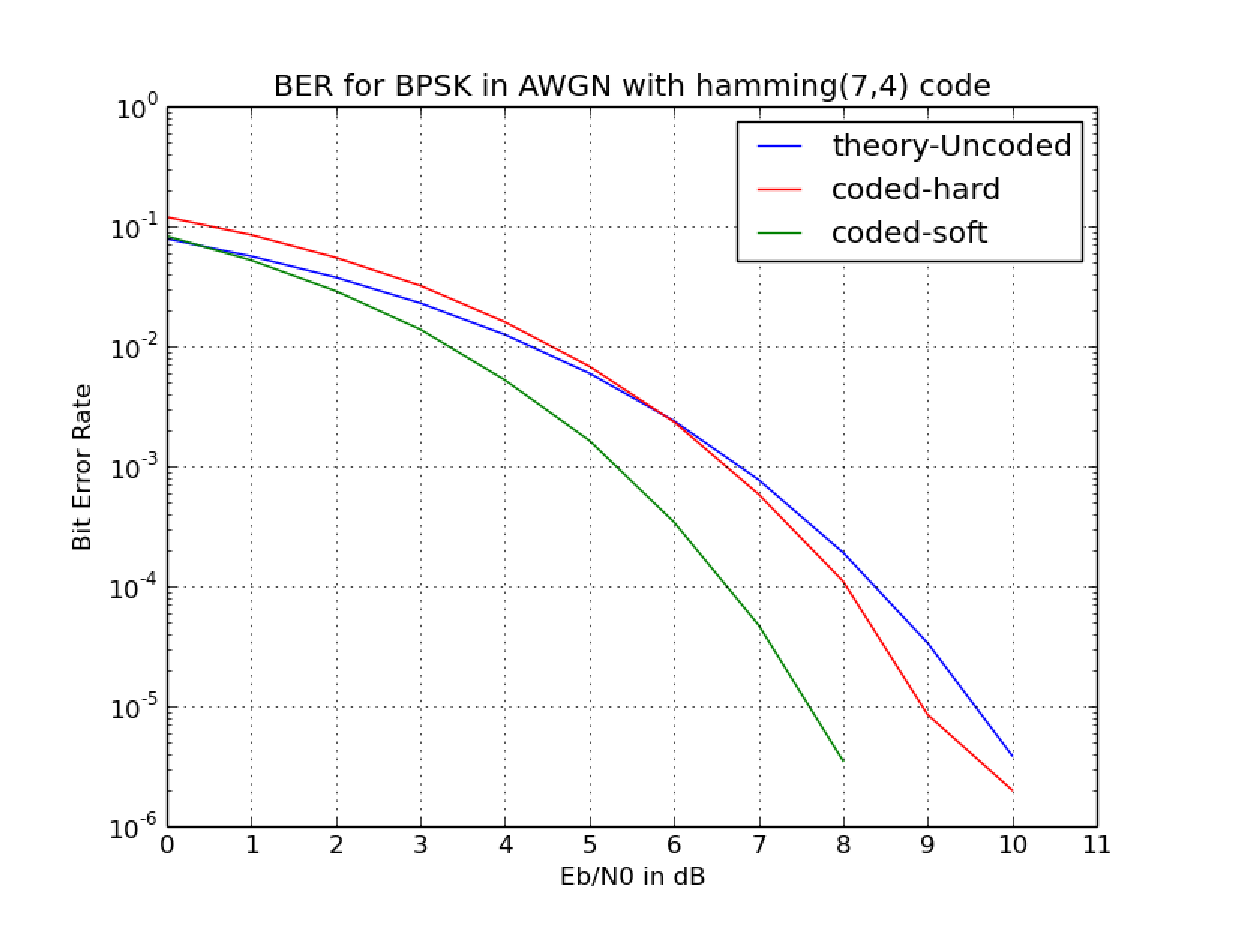
\includegraphics[width=\columnwidth]{./figs/BER_graph.eps}


\chapter{Convolution codes}


\section{Overview}

\Large{
The following code encodes the input data bits using convolution codes before sending them through an AWGN channel using BPSK modulation. Viterbi decoding algorithm is used to decode the received data. }

\section{Encoder}
\Large{
The encoder is defnied as a function below. The 3 shift reisters have a default state of 0. The first register is fed the input bit, and two Mod-2 adders are employed to get the output using the values stored in the other registers (The value stored in each register is shifted into the next register after each iteration).  }\\

\begin{minted}
[frame=lines,
bgcolor=mygray,
]
{python}
def conv_Encoder(conv_in): 
    m1=0
    m2=0
    m3=0
    len_msg=len(conv_in)
    conv_out=[]
    for i in range(len_msg):
        m1=conv_in[i]
        x1=m1^m3
        x2=m1^m2^m3 
\end{minted}
\\


\begin{minted}
[frame=lines,
bgcolor=mygray,
]
{python}
        conv_out.append(x1) 
        conv_out.append(x2)
        m3=m2
        m2=m1
    return conv_out
\end{minted}


\Large{
The SNR for coded and uncoded data is defined for N = $\mathrm{2}*10^6$ bits.}


\begin{minted}
[frame=lines,
bgcolor=mygray,
]
{python}
N=int(2e6)
Eb_N0_dB=np.arange(0,11,1)
Ec_N0_dB=Eb_N0_dB - 10*np.log10(2.0/1.0)
snrlen=11  
\end{minted}
\\

\Large{
The next part of the code generates the random data bits, encodes them and splits them into 2 data streams before applying BPSK modulation.  }\\

\begin{minted}
[frame=lines,
bgcolor=mygray,
]
{python}
for i in range(snrlen):
    ip = np.random.randint(2,size=N)
    conv_in=list(ip)
    #making last two data bits to zeros
    conv_in[N-1]=0
    conv_in[N-2]=0
    #Encoding the data
    conv_out=conv_Encoder(conv_in) 
    #divide encoded data into two streams
    conv1_out=conv_out[0:len(conv_out):2]
    conv2_out=conv_out[1:len(conv_out):2]
    #BPSK modulation
    conv1_mod=2*np.array(conv1_out)-1
    conv2_mod=2*np.array(conv2_out)-1  
\end{minted}
\\


\Large{
White Gaussian Noise is generated and added to the two signal streams.  }\\

\begin{minted}
[frame=lines,
bgcolor=mygray,
]
{python}
    sigma = np.sqrt((1/2.0)*(10**(-Ec_N0_dB[i]/10.0)))
    n1=np.random.normal(0,sigma,(np.shape(conv1_out)))  
    n2=np.random.normal(0,sigma,(np.shape(conv2_out)))  
    y1=conv1_mod+n1
    y2=conv2_mod+n2
\end{minted}
\\


\section{Decoder}
\Large{The received bits are decoded using the Viterbi decoder. The hard dcision Viterbi decoding algorithm finds the maximum likelihood estimate of the the transmitted sequence from the received sequence. The trellis diagram is used to compute the path metrics, as shown in the following figure.}\\ 


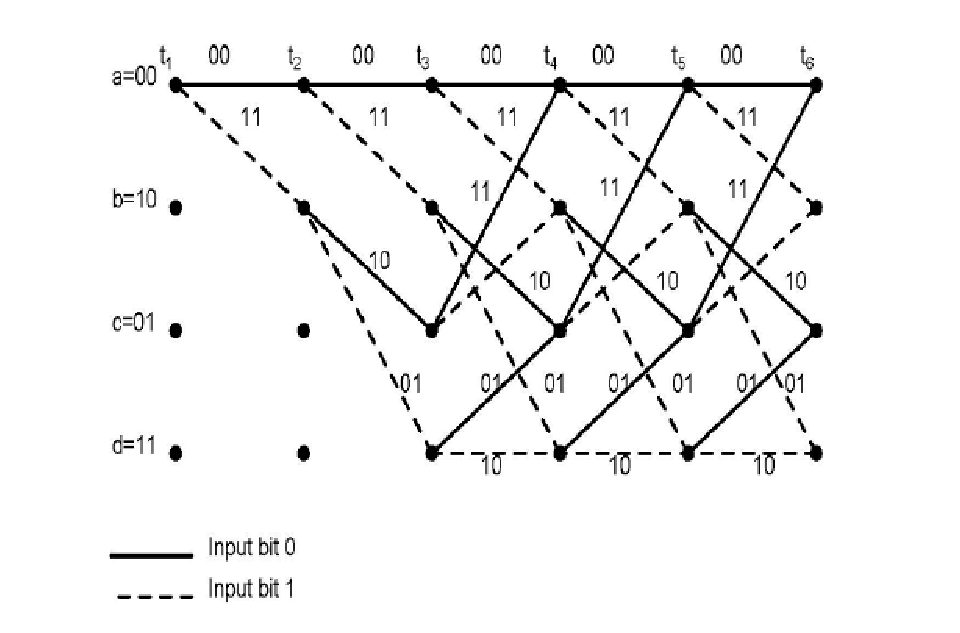
\includegraphics{./figs/trellis_diag.eps}


The viterbi decoder is defined in the following code. First, the 4 states are defined along with the distances and metrics.

\begin{minted}
[frame=lines,
bgcolor=mygray,
]
{python}
def viterbi(y1,y2,N):
    #number of states
    n=4
    #minimum distance to reach particular state
    distance=np.zeros((n,N+1))
    #initializing distances 
    distance[0:4,0]=[0,10e10,10e10,10e10]
    #metrics for transition from one state two another state
    metric=np.zeros((2*n,N))
\end{minted}
\\


\Large{The metrics for each possible transition are defined here, starting with the transition from the state 00 to 00, followed by 00 to 10, 10 to 01, 10 to 11, 01 to 00, 01 to 10, 11 to 01 and 11 to 11.}\\ 



\begin{minted}
[frame=lines,
bgcolor=mygray,
]
{python}
    for i in range(N):
        metric[0,i]=linalg.norm(np.array([-1,-1])
                    -np.array([y1[i],y2[i]]))
        metric[1,i]=linalg.norm(np.array([+1,+1])
                    -np.array([y1[i],y2[i]]))
        metric[2,i]=linalg.norm(np.array([-1,+1])
                    -np.array([y1[i],y2[i]]))
        metric[3,i]=linalg.norm(np.array([+1,-1])
                    -np.array([y1[i],y2[i]]))
        metric[4,i]=linalg.norm(np.array([+1,+1])
                    -np.array([y1[i],y2[i]]))
        metric[5,i]=linalg.norm(np.array([-1,-1])
                    -np.array([y1[i],y2[i]]))
        metric[6,i]=linalg.norm(np.array([+1,-1])
                    -np.array([y1[i],y2[i]]))
        metric[7,i]=linalg.norm(np.array([-1,+1])
                    -np.array([y1[i],y2[i]]))
\end{minted}
\\



\Large{Next the minimum distances to reach one of the four states is found for the \textit{i}th iteration. The distances are from the states 00, 10, 01 and 11 respectively. }\\ 


\begin{minted}
[frame=lines,
bgcolor=mygray,
]
{python}
        distance[0,i+1]=np.min([distance[0,i]+metric[0,i],
                        distance[2,i]+metric[4,i]])
        distance[1,i+1]=np.min([distance[0,i]+metric[1,i],
                        distance[2,i]+metric[5,i]])
        distance[2,i+1]=np.min([distance[1,i]+metric[2,i],
                        distance[3,i]+metric[6,i]])
        distance[3,i+1]=np.min([distance[1,i]+metric[3,i],
                        distance[3,i]+metric[7,i]])
\end{minted}
\\


\Large{
The following state space diagram is used as a reference for state transitions. The solid lines represent a state change when the input bit is \textit{0}, while the dotted line represent a state transition when the input is \textit{1}.
}

\begin{center}
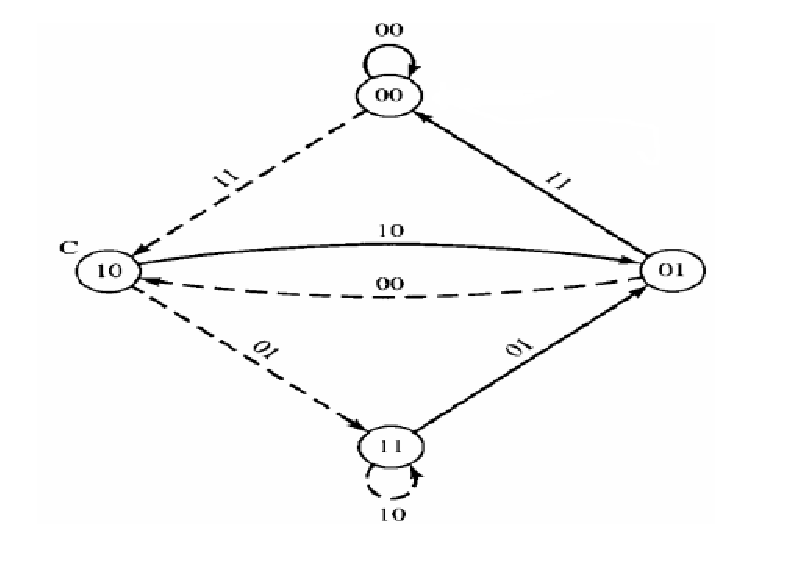
\includegraphics[scale=1]{./figs/enc_state_diag.eps}
\end{center}

\Large{
The currenct state or the final state is taken as a reference, and the distance and metric of the previous states are compared. Using the state space diagram above, the sum of the distance and metric is compared for each state and the decoded bit is deduced.
}\\


\begin{minted}
[frame=lines,
bgcolor=mygray,
]
{python}
    #Picking the state corresponding to minimum weight
    state=np.argmin(distance[:,N])   
    decoded_bit_final=np.zeros((N,))
    for j in range(N-1,-1,-1):
        distance_prev=distance[:,j]
        metric1=metric[:,j]
            curr_state=state
        if(curr_state==0):
            if(distance_prev[0]+metric1[0] <= 
               distance_prev[2]+metric1[4]):
                prev_state=0
                decoded_bit=0
            else:
                prev_state=2
                decoded_bit=0

\end{minted}
\\

\begin{minted}
[frame=lines,
bgcolor=mygray,
]
{python}
        elif(curr_state==1):
            if(distance_prev[0]+metric1[1] <=
               distance_prev[2]+metric1[5]):
                prev_state=0
                decoded_bit=1    
            else:
                prev_state=2
                decoded_bit=1
        elif(curr_state==2):
            if(distance_prev[1]+metric1[2] <= 
               distance_prev[3]+metric1[6]):
                prev_state=1
                decoded_bit=0
            else:
                prev_state=3
                decoded_bit=0
        elif(curr_state==3):
            if(distance_prev[1]+metric1[3] <= 
               distance_prev[3]+metric1[7]):
                prev_state=1
                decoded_bit=1
            else:
                 prev_state=3
                decoded_bit=1
        state=prev_state
            #Store the decoded bit in decode_bit_final
            decoded_bit_final[j]=decoded_bit 
    return decoded_bit_final
\end{minted}




\Large{
The received bits are decoded using the above defined function and the number of errors are calculated. Here \textit{nErr\_hard} is an array of zeroes defined outside the \textit{for} loop.
}


\begin{minted}
[frame=lines,
bgcolor=mygray,
]
{python}
    #convolution decoder
    decoded_bits=viterbi(y1,y2,N)
    #number of Errors for given Snr
    nErr_hard[0,i] = np.count_nonzero(decoded_bits-conv_in)
\end{minted}
\\



\section{BER}

\Large{The following part of the code is used to calculate the BERs for coded and uncoded data and subsequently plot them.}\\


\begin{minted}
[frame=lines,
bgcolor=mygray,
]
{python}
# Theoretical BER for uncoded in AWGN
theoryBer = 0.5*special.erfc(np.sqrt(10**(Eb_N0_dB/10.0))) 
# BER for coded in AWGN
simBer_hard = nErr_hard/float(N)
#plot graph of SNR vs coded and uncoded systems
plt.plot(Eb_N0_dB,theoryBer,'b',Eb_N0_dB,simBer_hard[0],'g')
plt.legend(['theory-Uncoded','coded-hard'],loc=1)
plt.yscale('log')
plt.ylabel('Bit Error Rate')
plt.xlabel('Eb/N0 in dB')
plt.title('BER for BPSK in AWGN with rate 1/2 convoution code')
plt.grid()
plt.show()
\end{minted}
\\

\Large{It can be clearly seen from the graph that BER is reduced significantly using Convolution coding.
}


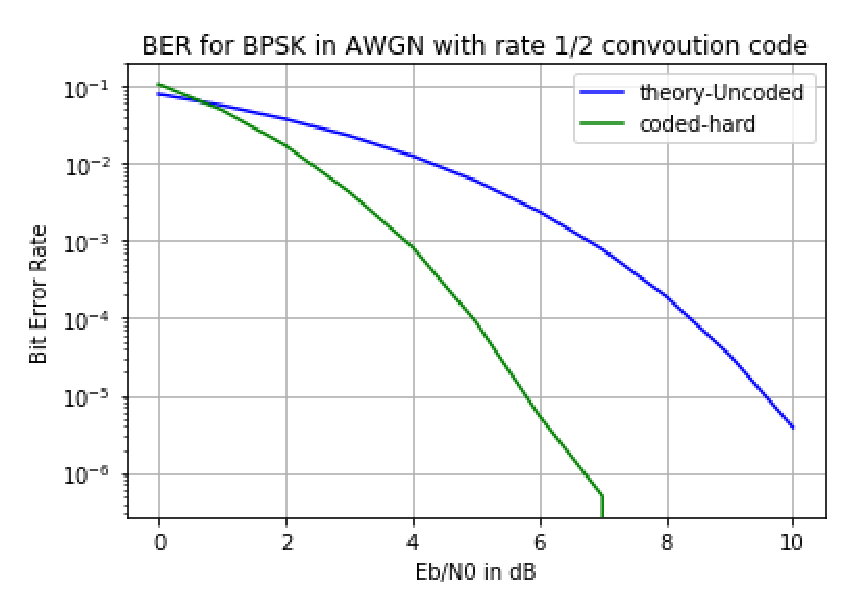
\includegraphics{./figs/BER.eps}


\end{document}